\subsection{Facade}

O \textit{pattern} Facade esconde toda a complexidade de uma ou mais classes do sistema e fornece uma interface, que o cliente pode aceder  para utilizar o sistema.

Ao se utilizar uma Facade, que implementa uma interface, pretende-se reduzir o nível de complexidade no subsistema, aumentando a facilidade de utilização.\\

\begin{figure}[!h]
\centering
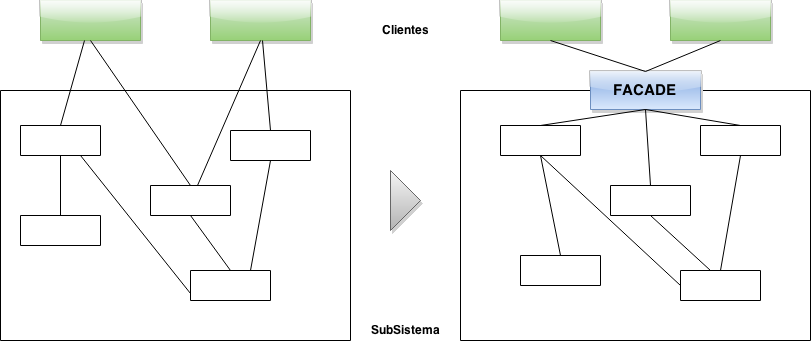
\includegraphics[scale=0.5]{img/facade-estrutura}
\caption{Antes e depois da utilização do Facade}
\end{figure}

Como vemos na figura anterior, este \textit{pattern} é definido através de uma única classe que fornece os métodos necessários ao cliente e envia os pedidos deste às classes do subsistema.\\

\textbf{Aplicação}

Utilizar Facade quando:

\begin{itemize}
  \item Se deseja fornecer uma interface simples para um sistema complexo.
  \item Existe muitas dependências entre clientes e as classes de implementação de uma abstração.
  \item Se pretende ter uma estrutura em camadas no sistema.\\
\end{itemize}

\textbf{Participantes}

\begin{description}
  \item[Facade] Sabe quais os tipos do subsistema são responsáveis por tratar um pedido, e portanto trata de gerir os pedidos entre o cliente e o subsistema.
  \item[Subclasses] Implementa as funcionalidades do subsistema. Desconhece a existência da classe Facade e responde aos pedidos feito por ela.\\
\end{description}

\textbf{Colaboração}

Os clientes comunicam com o subsistema através do envio de pedidos ao Facade, que redireciona os mesmos para as classes apropriadas do subsistema. Ainda que, os clientes que utilizam este \textit{pattern} não tem que aceder aos objetos do seu subsistema diretamente.\\

\textbf{Implementação}

\begin{figure}[!h]
\centering
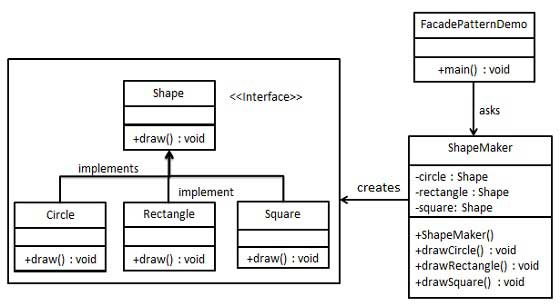
\includegraphics[scale=0.7]{img/facade_diagrama}
\caption{Diagrama de classe}
\end{figure}

Na estrutura anterior é criada uma interface \textit{Shape} que é implementada por as outras classes do subsistema.

A classe que define o Facade é a \textit{ShapeMaker} e é onde estão definidos os métodos que fornecem contacto aos clientes e as rotinas de gestão dos pedidos para o subsistema.

Por último, a classe \textit{FacadePatternDemo} será o cliente que faz pedidos à classe Facade definida anteriormente.\\

\textbf{Vantagens}

\begin{itemize}
\item A utilização deste \textit{pattern} permite diminuir as ligações entre os clientes e o sistema.
\item Para adicionar novas funcionalidades ao sistema seria necessário alterar apenas o Facade, ao invés de alterar os vários objetos do sistema, sem afetar o cliente.\\
\end{itemize}




